\documentclass[10pt,a4paper,twoside]{report}

%Configuration document

%%%%%%%%%%%%%%%%%%%%%%%%%%%%%%%%%%%%%%%%%%%%%%%%%%%%%%%%%%%%%%%%%%%%%%%%%%%%%%%
% PACKAGES
%%%%%%%%%%%%%%%%%%%%%%%%%%%%%%%%%%%%%%%%%%%%%%%%%%%%%%%%%%%%%%%%%%%%%%%%%%%%%%%

%Language
\usepackage[utf8]{inputenc} 			% Input encoding
\usepackage[english]{babel} 			% English

%Mathematics
\usepackage{amsmath}					% American Mathematical Society Package
\usepackage{amsfonts}					% Mathematical Fonts
\usepackage{amssymb}					% More mathematical symbols
\usepackage{mathtools}					% More control and better appearence of Mathematics

%Figures and captions
\usepackage{graphicx}					% More complex version of graphics for figures
\usepackage{caption}					% More control over captions
\usepackage{sidecap}					% Side captions (just in case)

%ThE LooOks!
\usepackage{fancyhdr}					% Fancy Headers
\usepackage{geometry}					% Control geometry
\usepackage{setspace}

%Tables and other enviorements
\usepackage{tabularx}					% Better tables
\usepackage{booktabs}					% Even better tables
\usepackage{enumitem}					% More control over enumerate enviorements
\usepackage{arydshln}					% Use dashed lines in tables

%Physics
\usepackage{siunitx}					% SI units			
\usepackage{physics}					% Usefull notations ( bras and kets for example)

% Usefull Tools
\usepackage{lipsum}						% Create random text
\usepackage{comment}					% Create comments
\usepackage{hyperref}					% Create hyperlinks
\usepackage{xcolor} 					% Colors
\usepackage{framed}						% Colored frames
\usepackage{setspace}					% Control spaces

%%%%%%%%%%%%%%%%%%%%%%%%%%%%%%%%%%%%%%%%%%%%%%%%%%%%%%%%%%%%%%%%%%%%%%%%%%%%%%%
% DOCUMENT SETUP
%%%%%%%%%%%%%%%%%%%%%%%%%%%%%%%%%%%%%%%%%%%%%%%%%%%%%%%%%%%%%%%%%%%%%%%%%%%%%%%

%Paper Geometry
\geometry{
	paper=a4paper, 	% A4 Paper
	inner=2.5cm, 	% Inner margin
	outer=2.5cm, 	% Outer margin
	top=2.5cm, 		% Top margin
	bottom=2.5cm, 	% Bottom margin
}

%Line spacing
\renewcommand{\baselinestretch}{1.5}

%Use Helvetica Font
\renewcommand{\rmdefault}{phv}
\renewcommand{\sfdefault}{phv}

\def\FontLn{% 16 pt normal
	\usefont{T1}{phv}{m}{n}\fontsize{16pt}{16pt}\selectfont}
\def\FontLb{% 16 pt bold
	\usefont{T1}{phv}{b}{n}\fontsize{16pt}{16pt}\selectfont}
\def\FontMn{% 14 pt normal
	\usefont{T1}{phv}{m}{n}\fontsize{14pt}{14pt}\selectfont}
\def\FontMb{% 14 pt bold
	\usefont{T1}{phv}{b}{n}\fontsize{14pt}{14pt}\selectfont}
\def\FontSn{% 12 pt normal
	\usefont{T1}{phv}{m}{n}\fontsize{12pt}{12pt}\selectfont}

%Mathematical font
\usepackage{sansmathfonts}

%Make tables align at the separator '.'
\usepackage{dcolumn}
\newcolumntype{d}{D{.}{.}{-1}}

%URL links setup
\colorlet{url_blue}{blue!50!black}

\hypersetup{
	pdfpagemode			= {UseOutlines}	,
	bookmarksopen		= true 			,
	bookmarksopenlevel	= 0				,
	hypertexnames		= false			,
	colorlinks			= true			, % Set to false to disable coloring links
	citecolor			= blue			, % The color of citations
	linkcolor			= blue			, % The color of references to document (sections, figures, etc)
	urlcolor			=url_blue		, % The color of hyperlinks (URLs)
	pdfstartview		={FitV}			,
	breaklinks			=true,
	unicode								,
}

%Setup sidecaption aligned to top of figure and caption width
\sidecaptionvpos{figure}{t}
\captionsetup{width=.8\textwidth}


%Set shaded color
\definecolor{shadecolor}{rgb}{0.8,0.8,0.8}

%%%%%%%%%%%%%%%%%%%%%%%%%%%%%%%%%%%%%%%%%%%%%%%%%%%%%%%%%%%%%%%%%%%%%%%%%%%%%%%
% COVER PAGE TOOLS
%%%%%%%%%%%%%%%%%%%%%%%%%%%%%%%%%%%%%%%%%%%%%%%%%%%%%%%%%%%%%%%%%%%%%%%%%%%%%%%

%new Latex variable names
\newcommand{\coverThesis}{@undefined} 
\newcommand{\coverSupervisors}{@undefined}
\newcommand{\coverExaminationCommittee}{@undefined}
\newcommand{\coverChairperson}{@undefined} 
\newcommand{\coverSupervisor}{@undefined} 
\newcommand{\coverMemberCommittee}{@undefined} 

\addto\captionsenglish{\renewcommand{\coverThesis}{Thesis to obtain the Master of Science Degree in}}
\addto\captionsenglish{\renewcommand{\coverSupervisors}{Supervisor}}
\addto\captionsenglish{\renewcommand{\coverExaminationCommittee}{Examination Committee}}
\addto\captionsenglish{\renewcommand{\coverChairperson}{Chairperson}}
\addto\captionsenglish{\renewcommand{\coverSupervisor}{Supervisor}}
\addto\captionsenglish{\renewcommand{\coverMemberCommittee}{Members of the Committee}}

%%%%%%%%%%%%%%%%%%%%%%%%%%%%%%%%%%%%%%%%%%%%%%%%%%%%%%%%%%%%%%%%%%%%%%%%%%%%%%%
% AKNOWLEDGMENT SECTION
%%%%%%%%%%%%%%%%%%%%%%%%%%%%%%%%%%%%%%%%%%%%%%%%%%%%%%%%%%%%%%%%%%%%%%%%%%%%%%%

% new LaTeX variable name
\newcommand{\acknowledgments}{@undefined} 
\addto\captionsenglish{\renewcommand{\acknowledgments}{Acknowledgments}}

%%%%%%%%%%%%%%%%%%%%%%%%%%%%%%%%%%%%%%%%%%%%%%%%%%%%%%%%%%%%%%%%%%%%%%%%%%%%%%%
% NOMENCLATURE AND GLOSSARY
%%%%%%%%%%%%%%%%%%%%%%%%%%%%%%%%%%%%%%%%%%%%%%%%%%%%%%%%%%%%%%%%%%%%%%%%%%%%%%%

\usepackage{nomencl}
\makenomenclature

% Group variables according to their symbol type
\RequirePackage{ifthen}

\renewcommand{\nomgroup}[1]{%
	\ifthenelse{	\equal{#1}{R}	}{	\item[\textbf{Roman symbols}]	}{%
	\ifthenelse{	\equal{#1}{G}	}{	\item[\textbf{Greek symbols}]	}{%
   	\ifthenelse{	\equal{#1}{S}	}{	\item[\textbf{Subscripts}]		}{%
  	\ifthenelse{	\equal{#1}{T}	}{	\item[\textbf{Superscripts}]	}{%   
  	}}}}}
    

%%%%%%%%%%%%%%%%%%%%%%%%%%%%%%%%%%%%%%%%%%%%%%%%%%%%%%%%%%%%%%%%%%%%%%%%%%%%%%%
% BIBLIO SETUP
%%%%%%%%%%%%%%%%%%%%%%%%%%%%%%%%%%%%%%%%%%%%%%%%%%%%%%%%%%%%%%%%%%%%%%%%%%%%%%%

\usepackage[backend=bibtex , style=chem-angew ,doi=false , url=false , isbn=false ]{biblatex}

%Bibligraphy file
\bibliography{./bib/my_ref} 


% Costumize color of bibliography
\newbibmacro{string+doiurl}[1]{%
	\iffieldundef{doi}
	{\iffieldundef{url}
		{#1}
		{\href{\thefield{url}}{#1}}}
	{\href{https://doi.org/\thefield{doi}}{#1}}}


\makeatletter

\def\blx@driver#1{%
	\ifcsdef{blx@bbx@#1}
	{\usebibmacro{string+doiurl}{\csuse{blx@bbx@#1}}}
	{\ifcsdef{blx@bbx@*}
		{\blx@warning{%
				No driver for entry type '#1'.\MessageBreak
				Using fallback driver}%
			\usebibmacro{string+doiurl}{\csuse{blx@bbx@*}}}
		{\blx@error
			{No driver found}
			{I can't find a driver for the entry type
				'\abx@field@entrytype'\MessageBreak
				and there is no fallback driver either}}}}
\makeatother




\begin{comment}
\usepackage[acronym,nonumberlist]{glossaries}
\makeglossaries

\usepackage{rotating}
\usepackage{xcolor}
\definecolor{YKblue}{rgb}{0.0, 0.18, 0.65}
\usepackage{hyperref}
\hypersetup{pdftitle={Terahertz plasmonic instabilities in graphene: a
hydrodynamical description},
            pdfauthor={Pedro A. Cosme S.},
            pdfsubject={Terahertz plasmonic instabilities in graphene: a
hydrodynamical description},
            pdfkeywords={Graphene plasmonic Thz emission},
            pdfstartview=FitV,
            pdfdisplaydoctitle=true,
            pdfpagemode=UseOutlines,
            urlbordercolor	=YKblue}



% 'hypcap' package
%
% Adjusting the anchors of captions.
% http://www.ctan.org/tex-archive/macros/latex/contrib/oberdiek/
%
% > fixes the problem with hyperref, that links to floats points
%   below the caption and not at the beginning of the float.
%
%\usepackage[figure,table]{hypcap}
%\usepackage{url}
%\usepackage[numbers,compress]{natbib} 
%\usepackage{notoccite}
%\usepackage{multirow}

\usepackage{booktabs}

%\usepackage{pdfpages}

%\usepackage{import}

% ----------------------------------------------------------------------
% Define new commands to assure consistent treatment throughout document
% ----------------------------------------------------------------------

%\newcommand{\ud}{\mathrm{d}}                % total derivative
%\newcommand{\degree}{\ensuremath{^\circ\,}} % degrees
% Abbreviations
%\newcommand{\mcol}{\multicolumn}            % table format
%\newcommand{\eqnref}[1]{(\ref{#1})}
%\newcommand{\class}[1]{\texttt{#1}}
%\newcommand{\package}[1]{\texttt{#1}}
%\newcommand{\file}[1]{\texttt{#1}}
%\newcommand{\BibTeX}{\textsc{Bib}\TeX}

% Typefaces ( example: {\bf Bold text here} )
%
% > pre-defined
%   \bf % bold face
%   \it % italic
%   \tt % typewriter
%
% > newly defined
%\newcommand{\tr}[1]{{\ensuremath{\textrm{#1}}}}   % text roman
%\newcommand{\tb}[1]{{\ensuremath{\textbf{#1}}}}   % text bold face
%\newcommand{\ti}[1]{{\ensuremath{\textit{#1}}}}   % text italic
%\newcommand{\mc}[1]{{\ensuremath{\mathcal{#1}}}}  % math calygraphy
%\newcommand{\mco}[1]{{\ensuremath{\mathcalold{#1}}}}% math old calygraphy
%\newcommand{\mr}[1]{{\ensuremath{\mathrm{#1}}}}   % math roman
%\newcommand{\mb}[1]{{\ensuremath{\mathbf{#1}}}}   % math bold face
%\newcommand{\bs}[1]{\ensuremath{\boldsymbol{#1}}} % math symbol
%\def\bm#1{\mathchoice                             % math bold
%  {\mbox{\boldmath$\displaystyle#1$}}%
%  {\mbox{\boldmath$#1$}}%
%  {\mbox{\boldmath$\scriptstyle#1$}}%
%  {\mbox{\boldmath$\scriptscriptstyle#1$}}}
%\newcommand{\boldcal}[1]{{\ensuremath{\boldsymbol{\mathcal{#1}}}}}% math bold calygraphy

\usepackage{nicematrix}
\usepackage{bigints}
\usepackage{cancel}
\usepackage{physics}
\usepackage{tikz}
\usepackage{ textcomp }
\usetikzlibrary{patterns,arrows,shapes,arrows,intersections,decorations,shadows,shapes.geometric}
\usepackage{tikz-3dplot}
\usepackage{circuitikz}
\usepackage{amsmath,amssymb,amsfonts}
\usepackage{verbatim}
\usepackage{cases}

\usepackage{caption}
\usepackage{subcaption}

%\usepackage[rightcaption]{sidecap}
%\sidecaptionvpos{figure}{t}


\newcommand{\secref}[1]{\S\ref{#1}}

\graphicspath{{./Figures/}{./Sections/}}

%\input{GFET.tex}
\captionsetup{width=.8\textwidth}





\end{comment}




\usepackage[acronym,nonumberlist]{glossaries}
\makeglossaries

\newglossaryentry{latex}
{
	name=latex,
	description={Is a mark up language specially suited
		for scientific documents}
}


\begin{document}

%%%%%%%%%%%%%%%%%%%%%%%%%%%%%%%%%%%%%%%%%%%%%%%%%%%%%%%%%%%%%%%%%%%%%%%%%%%%%%%
% FRONT MATTER
%%%%%%%%%%%%%%%%%%%%%%%%%%%%%%%%%%%%%%%%%%%%%%%%%%%%%%%%%%%%%%%%%%%%%%%%%%%%%%%

\pagestyle{plain}
\pagenumbering{roman}

% ----------------------------------------------------------------------
%  Cover , Dedication and Aknowledgements pages
% ----------------------------------------------------------------------

%Cover page

%%%%%%%%%%%%%%%%%%%%%%%%%%%%%%%%%%%%%%%%%%%%%%%%%%%%%%%%%%%%%%%%%%%%%%%%%%%%%%%
% COVER PAGE OF MASTER THESIS
%%%%%%%%%%%%%%%%%%%%%%%%%%%%%%%%%%%%%%%%%%%%%%%%%%%%%%%%%%%%%%%%%%%%%%%%%%%%%%%

\thispagestyle {empty}

%IST Logo

\includegraphics[viewport = 9.5cm 11cm 0cm 0cm ,scale = 0.29]{./inputs/01_Cover_Page/IST_A_CMYK_POS}

\begin{center}

% Figure (Image or plot)
\vspace{2.0cm}
%\includegraphics[height=50mm]{Figures/Airbus_A350.jpg}
\begin{center}

\includegraphics[height=40mm]{./inputs/01_Cover_Page/solomon}
\end{center}

% Thesis Title
\vspace{1.0cm}
{\FontLb A Master Thesis Template} \\ 
\vspace{0.2cm}
{\FontMn According to IST Regulations} \\
\vspace{0.9cm}

%Author name
\vspace{0.6cm}
{\FontMb John da Silva Smith} \\ 

%Degree
\vspace{2.0cm}
{\FontSn \coverThesis} \\
\vspace{0.3cm}
{\FontLb Engineering Physics}  \\

%Supervisors
\vspace{1.0cm}
{\FontSn %
\begin{tabular}{ll}
	\coverSupervisors: & Prof. Professor 1 \\
	                   & Prof. Professor 2
\end{tabular} } \\

%Examination Commitee
\vspace{1.0cm}
{\FontMb \coverExaminationCommittee} \\
\vspace{0.3cm}
{\FontSn %
\begin{tabular}{cc}
	  \coverChairperson:   &  Chairperson name  \\
	  \coverSupervisor:    &  Supervisor name   \\
	\coverMemberCommittee: & Committee Member 1 \\
	                       & Committee Member 1
\end{tabular} } \\

%Date of oral examination
\vspace{1.5cm}
{\FontMb Month 2021} \\ 


\end{center}

\cleardoublepage

%Dedication page

%%%%%%%%%%%%%%%%%%%%%%%%%%%%%%%%%%%%%%%%%%%%%%%%%%%%%%%%%%%%%%%%%%%%%%%%%%%%%%%
% DEDICATION PAGE
%%%%%%%%%%%%%%%%%%%%%%%%%%%%%%%%%%%%%%%%%%%%%%%%%%%%%%%%%%%%%%%%%%%%%%%%%%%%%%%

\null
\vskip5cm
\begin{flushright}
     Dedicated to Planet Earth\\
\end{flushright}
\vfill
\newpage
 
\cleardoublepage

%Aknowledgements page

\section*{\acknowledgments}

% Add entry in the table of contents as section
\addcontentsline{toc}{section}{\acknowledgments}

\lipsum[2] % 
\cleardoublepage

% ----------------------------------------------------------------------
%  %Abstract in mother language and english
% ----------------------------------------------------------------------

%Mother language

\section*{Resumo}

% Add entry in the table of contents as section
\addcontentsline{toc}{section}{Resumo}

\lipsum[2]


\vfill

\begin{tabular}{p{0.24\linewidth} p{0.6\linewidth}}
\textbf{\Large Palavras-chave:} & keyword 1; keyword  2; keyword 3  
\end{tabular}  \\   
\cleardoublepage

%English
\section*{Abstract}

% Add entry in the table of contents as section
\addcontentsline{toc}{section}{Abstract}

\lipsum[2]


\vfill

\begin{tabular}{p{0.24\linewidth} p{0.6\linewidth}}
	\textbf{\Large Keywords:} & keyword 1; keyword  2; keyword 3 
\end{tabular}  \\ 
\cleardoublepage


% ----------------------------------------------------------------------
%  Table of contents, list of tables, list of figures and nomenclature
% ----------------------------------------------------------------------

%Table of contents
\tableofcontents
\cleardoublepage 

%List of tables
\phantomsection
\addcontentsline{toc}{section}{\listtablename}
\listoftables
\cleardoublepage 

%List of figures
\phantomsection
\addcontentsline{toc}{section}{\listfigurename}
\listoffigures
\cleardoublepage 

%Nomenclature

% The definitions can be placed anywhere in the document body
% and their order is sorted by <symbol> automatically when
% calling makeindex in the makefile
%
% The \glossary command has the following syntax:
%
% \glossary{entry}
%
% The \nomenclature command has the following syntax:
%
% \nomenclature[<prefix>]{<symbol>}{<description>}
%
% where <prefix> is used for fine tuning the sort order,
% <symbol> is the symbol to be described, and <description> is
% the actual description.

% ----------------------------------------------------------------------
% Roman symbols [r]
\nomenclature[rE]{$\mathbf{E}$}{Electric field vector.}
\nomenclature[rB]{$\mathbf{B}$}{Magnetic field vector.}
\nomenclature[rS]{$\mathbf{S}$}{Poynting vector.}
\nomenclature[rL]{$\mathcal{L}$}{Lagrangian density.}
\nomenclature[rfour]{$\mathcal{F}[\quad]$}{Fourier transform.}
\nomenclature[rIm]{$\Im(\quad)$}{Imaginary part.}
\nomenclature[rRe]{$\Re(\quad)$}{Real part.}

% ----------------------------------------------------------------------
% Greek symbols [g]
\nomenclature[gh]{$\Theta(\quad)$}{Heaviside theta step function.}
\nomenclature[gs]{$\sigma$}{Conductivity.}
\nomenclature[gr]{$\rho$}{Mass density.}
\nomenclature[gy]{$\phi$}{Azimuthal angle.}
\nomenclature[gh]{$\theta$}{Polar angle.}
\nomenclature[gz]{$\omega$}{Frequency.}

% ----------------------------------------------------------------------
% Subscripts [s]
\nomenclature[s]{$x,y,z$}{Cartesian coordinates indices.}


% ----------------------------------------------------------------------
% Supercripts [t]
\nomenclature[t]{$\rm T$}{Transpose.}
\nomenclature[t]{$\dagger$}{Conjugate transpose (Hermitian conjugate).}
\nomenclature[t]{$\ast$}{Complex conjugate; adimensional quantity}
\nomenclature[t]{$k$}{Computational index for time step.}
\nomenclature[t]{$'$}{Derivative.}



\phantomsection
\addcontentsline{toc}{section}{\nomname}
\printnomenclature
\cleardoublepage

%Glossary
%exemplo de glossario em vez de acronimos
%\newglossaryentry{latex}
%{
        %name=latex,
        %description={Is a mark up language specially %suited for 
%scientific documents}
%}
\newacronym{ELT}{ELT}{Extremely Large Telescope} 
\newacronym{CERN}{CERN}{Conseil Européen pour la Recherche Nucléaire}  
\phantomsection
\addcontentsline{toc}{section}{\glossaryname}
\printglossary[type=\acronymtype , title=Acronyms]
\glsaddall

%%%%%%%%%%%%%%%%%%%%%%%%%%%%%%%%%%%%%%%%%%%%%%%%%%%%%%%%%%%%%%%%%%%%%%%%%%%%%%%
% MAIN MATTER
%%%%%%%%%%%%%%%%%%%%%%%%%%%%%%%%%%%%%%%%%%%%%%%%%%%%%%%%%%%%%%%%%%%%%%%%%%%%%%%

\setcounter{page}{1}
\pagenumbering{arabic}

% ----------------------------------------------------------------------
%  Chapters
% ----------------------------------------------------------------------


\chapter{Introduction}
\label{chapter:introduction}

\section{Section}


\lipsum[2]

\subsection{Subsection}

\lipsum[1]


%
\begin{equation}
S   = \int dt L
\end{equation}
%
\lipsum[3] 
%
\begin{equation}
\frac{d}{dt} \left( \frac{\partial L}{\partial \dot{q}_i} \right) - \frac{\partial L}{\partial q_i} = 0
\end{equation}
%
\lipsum[3]
\begin{equation}
L(t,q_i , \dot{q}_i) \rightarrow \mathcal{L}\left(x_\mu , \phi , \frac{\partial \phi}{\partial x_\mu} \right)
\end{equation}
%
\lipsum[3]
%
\begin{equation}
S = \int dt L = \int dx^4 \mathcal{L}	
\end{equation}
%
\lipsum[4]
%
\begin{equation}
\partial_\mu \left( \frac{\partial \mathcal{L}}{\partial (\partial_\mu \phi)}\right) - \frac{\partial \mathcal{L}}{\partial \phi} = 0
\end{equation}
%


\begin{figure}[ht!]
	\centering
	%   \resizebox{0.8\textwidth}{!}{
	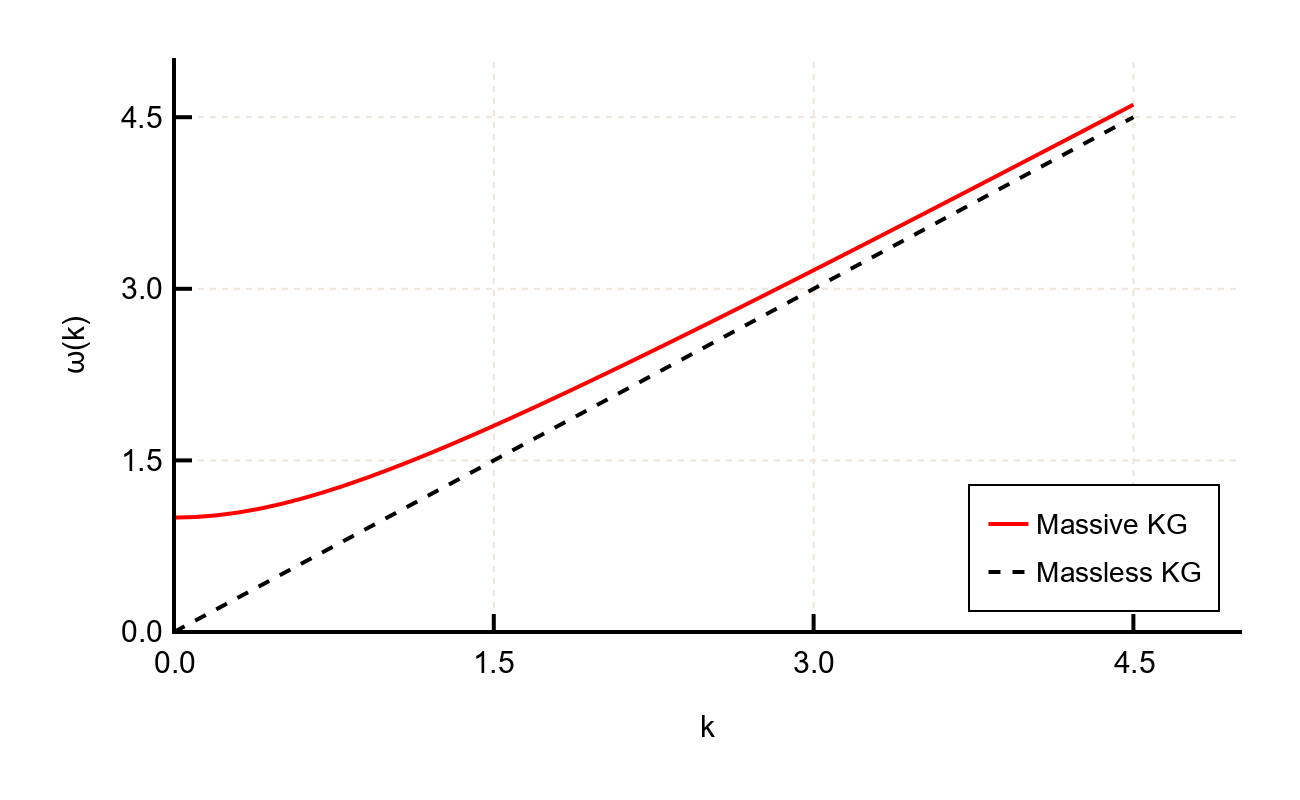
\includegraphics[width=0.8\linewidth]{figures/klein_gordon_DR}
	%    }
	\caption[Example figure 1]{ This is an example image with a caption }
	\label{fig:phasediagram_fluid}
\end{figure}




\subsection{Another Subsection}

\lipsum[1]

\subsubsection*{A Subsection without a number!}


\lipsum[3]

\begin{shaded}
	\textbf{Remark:}
	
	This is a block that can also be used for theorems, small notes...
	%
	\begin{equation}
	\eta_{\mu \nu} = ( - \;,\; + \;,\; + \;,\; +)
	\end{equation}
	
\end{shaded}

\lipsum[3]

\section{Last Section}

\lipsum[2]


\subsection{Example Table}
\lipsum[7]
%

\begin{table}[h]
\begin{center}
	\begin{tabular}{ ||p{3cm}|p{3cm}||p{3cm}|p{3cm}||  }
		\hline
		\multicolumn{4}{|c|}{\textbf{Table Title}} \\
		\hline
		\multicolumn{2}{||c||}{\textbf{Group I}} & \multicolumn{2}{c||}{\textbf{Group II}} \\
		\hline
		Parameter 1   	& 	1.0    	& Parameter 3		&   1.0	\\
		Parameter 2   	& 	27.0  	& Parameter 4   	&	0  	\\
		\hline
	\end{tabular}
  \captionsetup{width=14cm}

\caption{ An example table with a matching caption. If you change the size of the table, make sure to change the caption setup above }\label{tab:noPublications}
\end{center}
\end{table}

\lipsum[3]
\lipsum[3-5]

\begin{figure}[!hb]
	\centering
	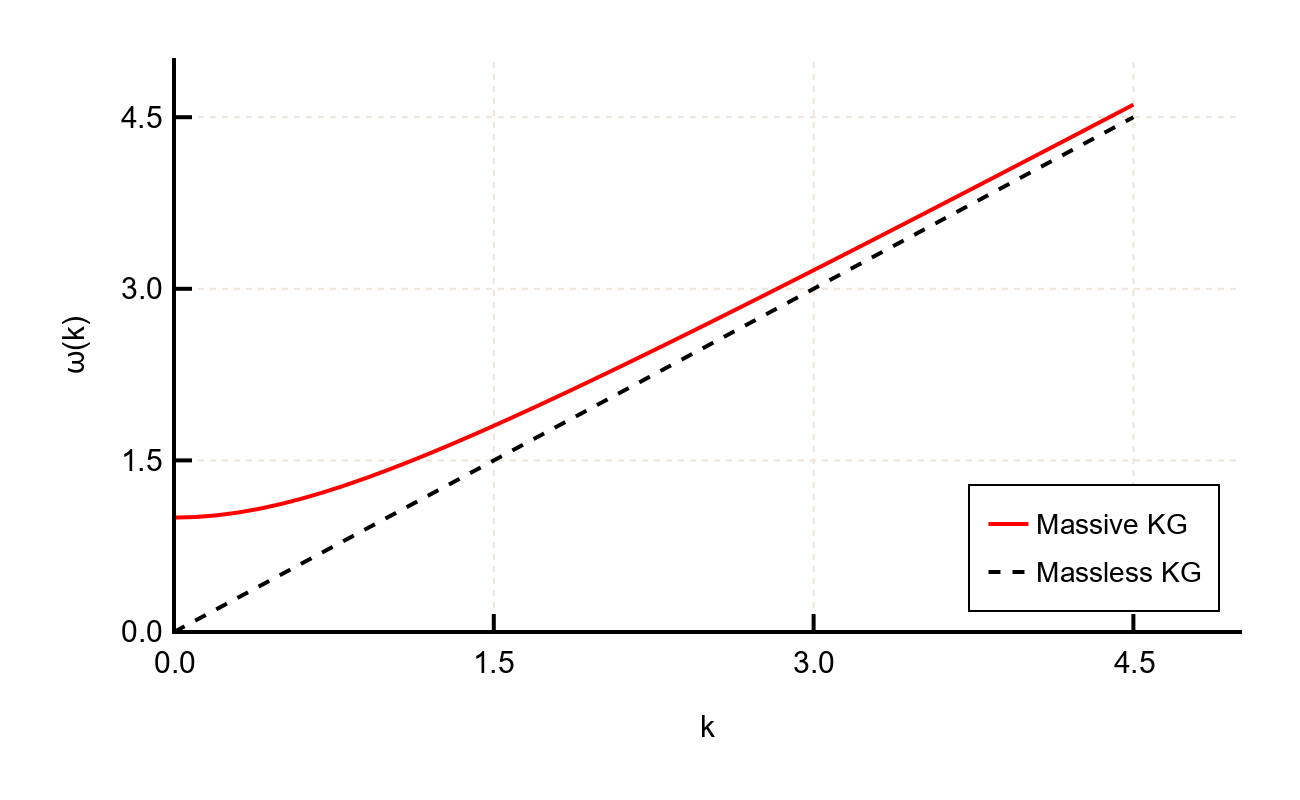
\includegraphics[width=0.8\textwidth]{figures/klein_gordon_DR}
	\caption[Example figure 2]{This is another example image with a longer caption. If the text is too long it wraps automatically underneath the figure. }
	\label{fig:richtmyerstencil}
\end{figure}


\cleardoublepage

% ----------------------------------------------------------------------
%  Bibliography
% ----------------------------------------------------------------------

\phantomsection
\addcontentsline{toc}{chapter}{\bibname}
\nocite{*}

\printbibliography
\cleardoublepage

%%%%%%%%%%%%%%%%%%%%%%%%%%%%%%%%%%%%%%%%%%%%%%%%%%%%%%%%%%%%%%%%%%%%%%%%%%%%%%%
% AFTER MATTER
%%%%%%%%%%%%%%%%%%%%%%%%%%%%%%%%%%%%%%%%%%%%%%%%%%%%%%%%%%%%%%%%%%%%%%%%%%%%%%%
\appendix

\chapter{Title of your appendix!}
\label{appEuler:derivation}

\lipsum[66]
\begin{equation}
    \mathcal{L}_{\mathcal{T}}(\vec{\lambda}) = \sum_{\mathbf{x},\mathbf{s}\in\mathcal{T}} \log P(\mathbf{x}|\mathbf{S}) - \sum_{i=1}^m \frac{\lambda_i^2}{2\sigma^2}
\end{equation}

\lipsum[66] 
\cleardoublepage

\end{document}